\documentclass[a4paper,12pt]{report} 
\usepackage[utf8x]{inputenc}
\usepackage[french]{babel}
\usepackage{mathtools}
\usepackage{amsmath}
\usepackage{amsfonts}
\usepackage{amssymb}
\usepackage{textcomp}
\usepackage[nointegrals]{wasysym}			% Collection de symboles mathématiques
\usepackage{multicol}					% Pour utiliser \hfill
\usepackage{ifthen}
\usepackage{tabularx}	 				% Gestion avancée des tableaux
%\usepackage{cleveref}

\usepackage{enumitem}
\usepackage{wrapfig}
%\usepackage[squaren]{SIunits}
%\usepackage[T1]{fontenc}				% Indispendable, présent dans tous les codes exemples
\usepackage[linkcolor=DarkGreen,colorlinks=true, citecolor= DarkGreen, urlcolor=MidnightBlue]{hyperref} 	% Hyper ref
\usepackage{listings}					% Pour citer du code
\usepackage[justification=centering]{caption}
\usepackage{sistyle} 
\usepackage{numprint}
\usepackage{wrapfig}
\usepackage{cite}	
\usepackage{url} 					% Pour citer les sites internet dans la
%\usepackage{cleveref}
\usepackage{setspace}

\usepackage{graphicx}		 			% Inclusion des figures
\graphicspath{{./pic/}}
\usepackage[svgnames]{xcolor}			%https://www.latextemplates.com/svgnames-colors

\newcommand{\bepar}[1]{
	\left( #1 \right)  
}

\newcommand{\becro}[1]{
	\left[ #1 \right]  
}

\newcommand{\rbk}[1]{\color{red}\textit{#1} \color{black}  
}

\usepackage{listings}					% Pour citer du code
%%%%%%%%%%%%%%%%%%%
%%% Élément pour citer des codes %%%
\lstset{
language=Python,
basicstyle=\ttfamily\bfseries\small, %
identifierstyle=\bfseries\color{black}, %
keywordstyle=\color{blue}, %
stringstyle=\color{black!90}, %
commentstyle=\it\color{black!70}, %
columns=flexible, %
tabsize=4, %
extendedchars=true, %
showspaces=false, %
showstringspaces=false, % %
numberstyle=\small, %
breaklines=true, %
breakautoindent=true, %
captionpos=b,
otherkeywords={cross_val_score},
keywords=[0]{cv},
keywordstyle=[0]{\color{red}},
}
%%%%%%%%%%%%%%%%%%%%%
\title{\navy \textbf{Notes Machine Learning} \color{black}}%%%%%%%%%%%%%%%%%%%%
\date{}
%\usepackage{multicol}
%\usepackage{etoolbox}
%\patchcmd{\thebibliography}{\section*{\refname}}
%    {\begin{multicols}{2}[\section*{\refname}]}{}{}
%\patchcmd{\endthebibliography}{\endlist}{\endlist\end{multicols}}{}{}
\usepackage[authoryear]{natbib}

\usepackage{geometry}
\geometry{hmargin=2cm, vmargin=2cm}

%%%%%%%%%%%%%%%%%%%%
%%% Couleurs %%%
\xdefinecolor{brick}{named}{DarkRed}
\xdefinecolor{navy}{named}{Navy}
\xdefinecolor{midblue}{named}{MidnightBlue}
\xdefinecolor{dsb}{named}{DarkSlateGray}
\xdefinecolor{dgreen}{named}{DarkGreen}

%%% 	Raccourcis 	%%%
\newcommand{\keps}{$k-\varepsilon$}
\newcommand\bk{\color{black}}
\newcommand\brick{\color{brick}}
\newcommand\navy{\color{navy}}
\newcommand\midblue{\color{midblue}}
\newcommand\dsb{\color{dsb}}
\newcommand{\dgreen}{\color{dgreen}}
\newcommand\red{\color{red}}

%%%%%%%% Cigles
\newcommand{\rap}{par rapport }
\newcommand{\cad}{c'est-à-dire}

%%%%%%%% Autres

%%%%%%%%%%%%%%%%%%%
% Syntax: \colorboxed[<color model>]{<color specification>}{<math formula>}
\newcommand*{\colorboxed}{}
\def\colorboxed#1#{%
  \colorboxedAux{#1}%
}
\newcommand*{\colorboxedAux}[3]{%
  % #1: optional argument for color model
  % #2: color specification
  % #3: formula
  \begingroup
    \colorlet{cb@saved}{.}%
    \color#1{#2}%
    \boxed{%
      \color{cb@saved}%
      #3%
    }%
  \endgroup
}
\renewcommand{\sectionmark}[1]{\markright{#1}}
\usepackage{fancyhdr}
\pagestyle{fancy}
\lhead{\textbf{Nathaniel} \brick \textbf{\textsc{Saura}}}
\rhead{\markright}
\cfoot{\thepage}
\renewcommand{\headrulewidth}{0.4pt}

\numberwithin{equation}{section} %%%% To count the equation like Section.Number



\begin{document}
\maketitle

\tableofcontents
\bibliographystyle{apalike}
\bibliography{bibliotheque}

\newpage 

\navy \chapter{NN VS GP} \bk
\cite{rasmussen2006gaussian} définissent le \textit{surpervised learning} comme l'apprentissage d'une correspondance entrées/sortie (on parlera de \textit{mapping}), à partir de données préalables. Ces données sont regroupées en paires dans un ensemble communément appelée Dataset : \\ 
\begin{equation}
\mathcal{D} = \left\{ \left( x_i, y_i \right) : i = 1,. . ., n \right\}
\end{equation}
\noindent Le procédé d'apprentissage (ou \textit{learning}), consiste à passer de $\mathcal{D}$, une connaissance \textit{spécifique}, à une connaissance \textit{généralisée} dans le but de \textit{mapper} n'importe qu'elle entrée avec une sortie cohérente, selon le problème étudié. On construit donc une fonctionnelle liant entrées et sorties. Cette fonctionnelle peut se construire de plusieurs façons. 
\section{Neural Networks}
L'approche Neural Network consiste à n'utiliser que des combinaisons linéaires des entrées de chaque couche. Chaque site recevant cette entrée émet ensuite un signal à la couche de neurones suivante. Ce signal est une fonction non linéaire de l'entrée (voir plus loin ou autres notes sur les différentes fonctions d'activation). \\
Mais de maniere générale les relations entre les entrées sont toujours linéaires.
\section{Processus Gaussien (régression)}

\begin{figure}[!ht]
\centering 
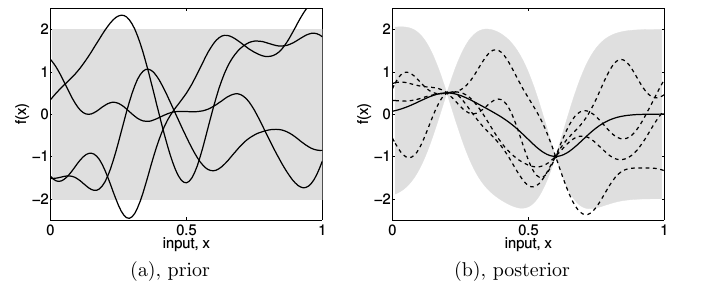
\includegraphics[scale=0.5]{fig_ramuss_1.png}
\caption{Provient de \citep{rasmussen2006gaussian}}
\label{ramuss_1}
\end{figure}

\noindent Cette idée généralise la notion de distribution Gaussienne (DG). De manière générale, lorsqu'une distribution de probabilité nous renseigne sur une \textbf{variable} ou un \textbf{vecteur} \textit{aléatoire}, un processus stochastique régit les \textit{propriétés} d'une distribution de \textbf{fonctions}. Sous des conditions particulières, les modèles de GP peuvent être mathématiquement équivalents aux splines, larges Neural Networks etc.. \\ 
D'une manière plus formelle un GP est une collection de variables aléatoires dont on peut trouver, pour n'importe quel nombre d'entre elles, une distribution jointe, gaussienne.\\
L'approche du processus Gaussien consiste à adapter la fonction liant les entrées. C'est-à-dire, initialement toutes les fonctions sont possibles, mais le processus Gaussiens nous permet de donner plus de poids à telle ou telle fonction en spécifiant les propriétés recherchées.\\
Même si initialement toutes les fonctions sont possibles, en choisir une en particulier n'influe pas sur le résultat final. Les GP permettent d'obtenir une connaissance claire sur les statistiques de données ainsi que sur les relations (linéaires, etc). On parlera de \textit{tracabilité} du calcul. \\

Si $m(\textbf{x})$ représente la moyenne du GP et $k\bepar{\textbf{x}, \textbf{x}'}$ sa covariance (ou plutôt sa fonction de covariance, voir plus loin), et qu'on note $f$ un tirage d'une telle distribution, on écrira :
\begin{equation}
f \sim \mathcal{GP}\bepar{m(\textbf{x}), k\bepar{\textbf{x}, \textbf{x}'}}
\end{equation}
Dans le manque d'informations (et de manière générale), on imposera une moyenne nulle pour tous les points\footnote{Cela n'implique pas forcément que chaque sample (ici ce sont des functions) a une moyenne nulle, mais que pour un nombre suffisant de tirage, la moyenne de ces fonctions en un point fixé est nulle.}. \\ 
La première étape consiste à fournir une distribution \textit{prior} fixant les propriétés des fonctions avec lesquelles il faudra composer. Comme illustré figure \eqref{ramuss_1}, les tirages de la distribution prior ne tiennent compte d'aucune contrainte si ce n'est la classe de fonctions considérée. \\
La majorité des caractéristiques de la distribution de fonctions est régie par la forme de la Covariance du Processus Gaussien (GPC). \\

Finalement le problème du \textit{learning} dans le GP c'est celui de trouver les bonnes propriétés sur la Covariance, de sorte que les fonctions issues de cette distribution collent parfaitement avec les données (qu'on peut voir comme des contraintes sur la distribution prior). De cette façon, on obtient des propriétés sur les informations a posteriori que l'on peut interpréter. \\ Notons enfin que le GP nécessite d'inverser des covariances dont la taille est définie par la taille de la base de données utilisée, ce qui peut considérablement ralentir les calculs (par rapport au NN et la back propagation). \\[3mm]

\dgreen \textbf{\large{Exemple :}} \bk Supposons que l'on veut considérer uniquement des fonctions qui passent par deux points $A_1 = \left( x_1, y_1 \right)$ et $A_2 = \left( x_2, y_2\right)$. Le résultat du GP correspondant est illustré figure \eqref{ramuss_1}. On peut également rajouter une variabilité autour de ces points.\\
On remarque sur cette figure, que l'incertitude (zone grisée) est nulle aux points $A_1$ et $A_2$ et est maximale aux points les plus éloignés de $A_1$ \textsc{et} $A_2$.\\
La ligne solide représente la moyenne des tirages (lignes en pointillées), cette moyenne est consistente avec la contrainte initiale; elle constitue l'information \textit{a posteriori}.\\


\noindent Passer de $\mathcal{D}$ à la fonctionnelle $f$ se fait au travers l'apprentissage. On arrange les entrées $x_i$ en une matrice $\textbf{\textit{X}}$ de taille \textit{D}$\, \times \,n$ où \textit{D} représente la taille des données. Cette matrice est appelée \textit{design matrix}.\\
On concatène toutes les sorties en un seul vecteur $\vec{\textbf{y}}$, de telle sorte qu'on écrira 
\begin{equation}
\mathcal{D} = \bepar{\textit{\textbf{X}}, \vec{\textbf{y}}\,}
\end{equation}
Enfin déduire une fonctionnelle liant entrées et sorties revient à établir une distribution de probabilités conditionnelle donnant la sortie sachant l'entrée :
\begin{equation}
P \bepar{S | E}
\end{equation}

\brick \subsection{Learning en utilisant des poids} \bk
\subsubsection*{Retour sur le modèle linéaire : régression Baysienne}
\noindent Les modèles linéaires se basent sur une prédiction telle que
\begin{equation}
f(\textbf{x}) = \textbf{x}^T\textbf{w} \text{\hspace{1cm}(le biais est inclus)}
\end{equation}
La valeur observée, elle, s'écrit 
\begin{equation}
y = f(\textbf{x}) + \varepsilon
\end{equation}
On suppose que $y$ et $f(\textbf{x})$ diffèrent de $\varepsilon$, un bruit suivant une distribution Gaussienne (DG) indépendamment de $\textbf{x}$ ou $y$, de moyenne nulle et de variance $\sigma^2_n$. On écrit alors 
\begin{equation}
\varepsilon \sim \mathcal{N}\bepar{0, \sigma^2_n}
\end{equation}
Pour chaque paire $\bepar{x_i, y_i}$ le bruit $\varepsilon_i$ correspondant est indépendant de tous les autres indices. Ainsi, on peut exprimer la fonction de vraisemblance (\textit{likelihood function LF}) \textit{i.e.} la probabilité conditionnelle d'obtenir les sorties $\textbf{y}$ donnés $\textbf{\textit{X}}$ et $\textbf{w}$ :
\begin{equation}
L = p\bepar{\textbf{y} | \textbf{\textit{X}},\, \textbf{w}} =  \prod_{i=1}^{n} p\bepar{y_i | \textbf{x}_i, \, \textbf{w} }
\end{equation}
Cette dernière équation revient à multiplier les distributions Gaussiennes soit
\begin{equation}
\prod_{i=1}^n\frac{1}{\sqrt{2 \pi} \sigma_n} \exp{\bepar{- \frac{\bepar{y_i - \textbf{x}_i^T \textbf{w}}^2}{2 \sigma_n^2}}} 
\end{equation}
Ce produit revient à sommer les arguments des exponentielles et multiplier les termes en $\bepar{2\pi\sigma_n^2}^{1/2}$. Finalement, on peut reconnaitre (à un facteur près) en $L$ une DG autour de \textbf{y}:
\begin{equation}
L \sim \mathcal{N}\bepar{\textbf{\textit{X}}^T\textbf{w}, \, \sigma^2_n \textbf{\textit{I}}_n} \label{likely}
\end{equation}
Dans la théorie Baysienne, il faut spécifier une première estimation pour $\textbf{w}$. On suppose qu'il suit une DG : \begin{equation}
\textbf{w} \sim \mathcal{N}\bepar{0,\, \Sigma_p} \propto \exp{\bepar{-\frac{1}{2} \textbf{w}^T \Sigma^{-1}_p\textbf{w}}}
\end{equation}.\\
L'idée ici est d'utiliser le théorème de Bayes pouvant s'écrire :
\begin{equation}
\text{posterior} = \frac{\text{likelihood}\times\text{prior}}{\text{marginal likelihood}} \label{bayesTH}
\end{equation}
Ici on cherche à estimer les bonnes valeurs de \textbf{w}. La probabilité notée \textsc{posterior} fait allusion à $p\bepar{\textbf{w}|\textbf{\textit{X}}, \, \textbf{y}}$. \\
On définit également la fonction de probabilité conditionnelle \textit{marginal likelihood} qui est la somme de $L$ sur tous les poids possibles :
\begin{equation}
p\bepar{\textbf{y}|\textbf{\textit{X}}} = \int p\bepar{\textbf{y} | \textbf{\textit{X}},\, \textbf{w}} p\left( \textbf{w}\right ) d\textbf{w} 
\end{equation}

\noindent On peut alors exprimer \eqref{bayesTH} voir \citep{rasmussen2006gaussian}
\begin{equation}
\text{posterior} = p\bepar{\textbf{w}|\textbf{\textit{X}}, \, \textbf{y}} \sim \mathcal{N}\bepar{\sigma_n^{-2} A^{-1}\textbf{\textit{X}} A, \, A^{-1}} \text{\hspace{2mm} avec \hspace{2mm}} A = \sigma_n ^{-2} \textbf{\textit{X}}\textbf{\textit{X}}^T + \Sigma_p^{-1} \label{pwxy}
\end{equation}
La moyenne est appelée estimation \textit{maximum a posteriori} ou encore MAP de $\textbf{w}$. 

\noindent Ici on peut estimer la distribution de prédiction et donner sa nature grâce à \eqref{pwxy}: on note $f_*$ la prédiction $f(x_*)$ avec $x_*$ un élément extérieur au \textit{test set}. \\ On cherche alors la probabilité de trouver $f_*$ sachant $x_*$ et $\textbf{\textit{X}}$ ainsi que $\textbf{y}$ (mais pas \textbf{w} $(\neq$ NNs)). \\
Trouver cette probabilité revient finalement à trouver le meilleur set $\textbf{w}$ sachant $\textbf{\textit{X}}$ et $\textbf{y}$.\\
On va donc sommer sur $\textbf{w}$ toutes les estimations de $f_*$ sachant $x_*$ et \textbf{w}, en pondérant à chaque itération par la probabilité d'obtenir \textbf{w} sachant $\textbf{\textit{X}}$ et $\textbf{y}$. On écrit cette prédiction comme :
\begin{align}
p\bepar{f_*|x_*, \, \textbf{\textit{X}}, \, \textbf{y}} &= \int p\bepar{f_*|x_*,\, \textbf{w}} p\bepar{\textbf{w}|\textbf{\textit{X}}, \, \textbf{y}} d\textbf{w} = \int \textbf{x}_*^T\textbf{w} ~ p\bepar{\textbf{w} | \textbf{\textit{X}}, \, \textbf{y}} \label{predict}\\
&= \mathcal{N}\bepar{\sigma_n^{-2}\textbf{x}_*^TA^{-1}\textbf{\textit{X}}\textbf{y}, \, \textbf{x}_*^T A^{-1} \textbf{x}_*} \label{predict_DG}
\end{align}
Dans le membre du milieu de \eqref{predict}, on distingue deux termes : le premier $p\bepar{f_*|x_*,\, \textbf{w}}$ représente la probabilité d'avoir $f_*$ sachant $x_*$ et le poids $\textbf{w}$. Cette probabilité est pondérée par celle d'avoir $p\bepar{\textbf{w}|\textbf{\textit{X}}, \, \textbf{y}}$ \cad $ $ le taux de correspondance entre les poids \textbf{w} et les données de l'apprentissage.\\
Ainsi, ce sont bien les poids définies lors de la phase de training qui seront utilisés.\\
L'équation \eqref{predict_DG} nous renseigne quant à elle, sur la nature de la distribution prédite, elle est Gaussienne.

\subsubsection*{Projection dans l'espace des caractéristiques}
Pour augmenter les possibilités du modèle, on peut projeter les entrées dans un espace de plus grande dimension, appelée \textit{feature space}. On peut prendre l'exemple d'un scalaire $x$ projeté dans l'espace des puissances $\left( 1, x, x^2, x^3,...\,  \right )$.\\
On s'assure que le problème projeté reste bien linéaire tant que les projections sont indépendantes de $\textbf{w}$.\\ 
On substitue alors à $x$ : $\phi(x)$, ce qui nous permet d'écrire entre autres 
\begin{equation}
f(x) = \phi(x)^T\textbf{w}
\end{equation}
De manière analogue à ce qu'on a fait avec $\textbf{\textit{X}}$ on construit $\Phi(x)$ en concaténant en colone (cette fois) les $\phi(x)$ pour tous les cas de l'ensemble des tests.\\
Par la suite, on reprend \eqref{predict_DG} et on remplace $\textbf{x}_*$ et \textbf{\textit{X}} par $\phi(x_*)$ et $\Phi$ resp. :

\begin{equation}
p\bepar{f_*|\textbf{x}_*,\, \textbf{\textit{X}},\textbf{y}} \sim \mathcal{N}\bepar{\sigma_n^{-2}\phi(\textbf{x}_*)^TA^{-1}\Phi\textbf{y}, \, \phi(\textbf{x}_*)^T A^{-1} \phi(\textbf{x}_*)}
\end{equation}
On remanie cette équation pour éviter d'avoir à inverser la matrice  $A$ :
\begin{equation}
p\bepar{f_*|\textbf{x}_*,\, \textbf{\textit{X}},\textbf{y}} \sim \mathcal{N}\bepar{\phi_*^T \Sigma_p \Phi(K + \sigma_n^2 \textbf{ \textit{I}})^{-1}, \, \, \textsc{cov}} \label{distrib_FS}
\end{equation}
avec :
\begin{align}
K = \Phi^T \Sigma_p\Phi& \\
\textsc{cov} = \phi_*^T\Sigma_p\phi_* - \phi^T\Sigma_p\,\Phi&\left(K  + \sigma_n^2\mathbf{\mathit{I}}\right)^{-1}\Phi^T \Sigma_p\phi_* \label{covFS}
\end{align}
On remarque dans les expressions \eqref{distrib_FS} et \eqref{covFS} laprésence des termes $\displaystyle \phi_*^T\Sigma_p\phi_*\, \Phi^T\Sigma_p\Phi$ et $\phi_*^T\Sigma_p\Phi$. On peut poser $\displaystyle k(\textbf{x}, \textbf{x}') = \phi(x)^T\Sigma_p\phi(x')$, fonction qui s'appelle \textit{kernel} ou \textit{fonction de covariance}. De plus, dans le cas ou $\Sigma_p$ est définie positive, on peut poser $\displaystyle \psi(\textbf{x}) = \Sigma_p^{1/2} \phi(x)$ de telle sorte que
\begin{equation}
k(\textbf{x}, \textbf{x'}) = \psi(x)\cdot \psi(x')
\end{equation}
On reviendra sur ce \textit{kernel trick}.\\

\noindent Cette exemple de régression Baysienne nous permet de donner un exemple de GP : en prenant $f = \phi(\textbf{x})^T\textbf{w}$ avec $w \sim \mathcal{N}\bepar{0, \sigma_p}$, on peut calculer $\mathbb{E}[f(\textbf{x})]$ et $\mathbb{E}[f(\textbf{x})f(\textbf{x}')]$ correspondant à la moyenne et à la variance de $f$ :
\begin{align*}
\mathbb{E}[f(\textbf{x})] & = \phi(\textbf{x})\mathbb{E}[\textbf{w}] = 0 \\
\mathbb{E}[f(\textbf{x})f(\textbf{x}')] & = \phi(\textbf{x})^T \mathbb{E}[\textbf{w}\textbf{w}^T]\phi(\textbf{x}') = \phi(\textbf{x})^T \Sigma_p \, \phi(\textbf{x}')
\end{align*}
On retrouve alors l'\textit{inner product} $\phi(\textbf{x})^T \Sigma_p \, \phi(\textbf{x}')$.\\
Comme on l'a dit les fonctions de covariance (FDC) sont capitales pour que notre méthode se basant GP puisse apprendre et prédire avec précision. \\
Une de ces fonctions est la \textit{Radial Basis Function (RBF)} appelée également \textit{Squared Exponential (SE)}. On l'écrit :
\begin{equation}
 \textsc{cov}\bepar{f(\textbf{x}_p), \, f(\mathbf{x}_q)} = k\bepar{\textbf{x}_p, \textbf{x}_q} = \exp{\bepar{-\frac{1}{2}\left| \textbf{x}_p  - \textbf{x}_q\right|^2}}\label{RBF}
 \end{equation} 
Cette fonction permet de construire une covariance sur les sorties ($f_i$) en fonction des entrées. Plus les entrées sont éloignées, plus la covariance sera faible, alors que si les entrées sont très proches, cette covariance sera proche de l'unité.\\
La RBF en particulier est la fonction de covariance correspondant au model de régression Baysienne dont l'espace des caractéristiques est infinie. On peut également l'obtenir en considérant un nombre infini de combinaisons linéaires de fonction de bases de forme Gaussienne (Rajouter les ref chjap 4 eq 4.13 4.13 et Th section 4.3).\\
Avant de regarder dans les détails les fonctions de covariance, on peut remarquer que la FDC \eqref{RBF} est indéfiniment dérivables, on s'attendra alors à des tirages de fonctions lisses et continues.\\
De même, on peut ajuster la vitesse de variabilité des fonctions en normalisant la distance entre deux entrées.

\subsubsection*{Prédiction en utilisant des observations bruitées}
Dans ce cas, le training comprend des données dont la sortie est bruitée (incertitudes expérimentales, approximations ...). On en revient alors à écrire $y = f(\textbf{x}) + \varepsilon$. Avec la RBF, on peut écrire la covariance comme \eqref{RBF}, et puisque les bruits sont indépendants et aléatoires, les variances s'ajoutent. On a donc 
\begin{equation*}
\textsc{cov}\bepar{\textbf{y}_p, \textbf{y}_q} = k\bepar{\textbf{x}_p, \textbf{x}_q} + \sigma_n^2 \delta_{pq}
\end{equation*}
En évaluant $k\bepar{\textbf{x}_p, \textbf{x}_q}$ sur l'ensemble du training set, on peut écrire l'équation précédente sous forme matricielle :
\begin{equation}
\textsc{cov}(\textbf{y}) = K\bepar{\textbf{X}, \textbf{X}} + \sigma_n^2\textbf{\textit{I}}
\end{equation}
Les distributions de $\textbf{y}$ et de $\textbf{f}_*$ la prédiction s'écrit :
\begin{equation}
\left[ \begin{array}{c} 
 \textbf{y} \\ \textbf{f}_* \end{array}
\right] = \left[\begin{array}{c@{\qquad}c} K\left(\textbf{X}, \textbf{X}\right) + \sigma_n^2\textbf{\textit{I}}& K\bepar{\textbf{X}, \textbf{X}_*}\\ K\bepar{\textbf{X}_*, \textbf{X}} & K\bepar{\textbf{X}_*, \textbf{X}_*}\\  \end{array}\right]
\end{equation}
Avec l'indice $_*$ lorque que la quantité le portant se réfère à de la prédiction.\\

On peut alors doner l'équation clé de la prédiction pour un Processus Gaussien, dans un cas de régression : 
\begin{equation}
f_*|X,y,X_* \sim \mathcal{N}\bepar{\overline{f}_*, \textsc{cov}\left (f_*\right )}
\end{equation}
On simplifie les expressions de $\overline{f}_*$ et de $\textsc{cov}\left (f_*\right )$ en introduisant les notations suivantes
\newpage



\subsection{Notions}
\begin{itemize}
\item[--] \textbf{Le formalisme Bayesien} : consiste à estimer la probabilité d'un événement sachant la réalisation d'un autre. Dès lors que l'adjectif Bayesien est utilisé, il faut avoir en tête que de tels concepts sont mis en jeu. Le théorème de Bayes est le résultat de référence dans ce genre de problème. Les résultats et propriétés des probabilités conditionnelles sont également mis en jeu.
\item[--] \textbf{Homoscédasticité} : Une des hypothèses fondamentales de la régression linéaire. \\
Se dit lorsque la variance des erreurs stochastiques de la régression est la même pour chque observation : $\displaystyle \text{\textbf{Var}}[\varepsilon_i] = \sigma^2, \, \forall i$.
\item[--] \textbf{Hétéroscédasticité} : Variance des variables est différente (s'oppose à l'homoscédasticité) : $\displaystyle \text{\textbf{Var}}[\varepsilon_i] = \sigma_i^2$ par forcément égale à $\sigma_j^2$ pour $i \ne j$.
\end{itemize}

\section{Notes ML : \cite{muller2016introduction}}
\brick \subsection{Classification}\bk
\subsubsection{Binaires}
\navy \paragraph*{LogisticRegression} :\bk \\
\noindent Mesure la similitude entre une donnée et les classes avec une norme euclidienne.\\
Utilise la fonction logistique $f$ qui associe à toute entrée, valeur comprise entre 0 et 1.\\
Lors du training, sont déterminées les valeurs de $a$ et $b$ qui apparaissent dans le calcul de la «probabilité d'appartenance» d'une donnée à une des deux classes : $P = f\bepar{a+bx}$\\

\noindent Lors du training, on peut pénaliser \cad $ $ décomplexifier le training set pour améliorer les prédictions. Cette amélioration est due au fait qu'en pénalisant, on empêche le modèle de prendre en compte le bruit dans les données, les exceptions ou les particularités.
\subsubsection{Regression}
\brick \subsection{Évaluer son modèle : Cross Validation (CV)} \bk
\subsubsection{CV et Stratification (SCV)}
\textit{k-fold cross-validation} : k nombre de partitions voulues. Ces partitions ont approximativement la même taille et sont appelées \textit{folds}. À chque «tour», on reserve $1$ partition pour le test et on consacre les $k-1$ partitions restantes pour le training.
À chacun de ces cas, on calcule le score sur le test set. Pour avoir une meilleure idée de la capacité de production du modèle qu'avec model.score ou model.predict\_proba, on pourra prendre la moyenne des scores des différents \textit{folds}.
\begin{lstlisting}
	scores = cross_val_score(logreg, iris.data, iris.target, cv=5)	
	Cross validation scores : [ 1., 0.96666667, 0.93333333, 0.9, 1. ]	
	Average cross-validation score : 0.96
\end{lstlisting}

\noindent Cette méthode permet d'avoir une meilleure vue d'ensemble de la base de données puisque l'on a accès aux différents scores des \textit{folds}.
Cela nous renseigne aussi sur la sensitivité du modèle (overfitting) et sur les meilleurs ou pires scénarii possibles.\\
On optimise l'utilisation des données puisqu'on n'est plus limité au 80-20 du train\_test\_split.\\
Évidemment, le coût de calcul est aussi plus élevé. \\
Pour les classifier, il est recommandé d'utiliser la stratification puisqu'elle préserve les proportions des différentes classes pour la découpe de \textit{folds} et donc augmente la capacité de généralisation du modèle. Pour les problèmes de regression, cela n'a pas de sens.\\

\subsubsection{KFold CV}
On peut ensuite construire une cross validation pour mieux contrôler ce qu'il se passe pendant la séparation.
On utilise le \textit{splitter} Kfold. Ces trois arguments sont \color{red}\textit{n\_splits} \bk qui correspond au nombre de \textit{folds} voulu, \color{red} \textit{shuffle} \bk qui est un booléen et \color{red}\textit{random\_state} \bk qu'on fixera à zéro pour avoir des résultats reproductibles. On initialsera \color{red} cv \bk à kfold :
\begin{lstlisting}
from sklearn.model_selection import KFold
kfold = KFold(n_splits=3, shuffle=True, random_state=0)
scores = cross_val_score(logreg, iris.data, iris.target, cv=kfold)
Cross validation - KFold embedded scores : [ 0.9   0.96  0.96]
\end{lstlisting}

\subsubsection{Suffle Split CV (SSCV)}
On définit \rbk{train\_size} et \rbk{test\_size} respectivement la taille des éléments du training et de celle de ceux du test. On splitera en \rbk{n\_splits} la base de données et on sélectionnera aléatoirement \rbk{train\_size} élements du split comme étant la training  et les \rbk{test\_size} comme étant réservé pour le test.\\
On pourra éventuellement réitérer cette procédure. On pourra également ne considérer qu'une partie de la base de données.
\begin{lstlisting}
from sklearn.model_selection import ShuffleSplit
SSCV	=   ShuffleSplit(test_size = 0.5, train_size = 0.5, n_splits = 10)
SSCV scores : 
[ 0.96        0.90666667  0.96        0.94666667  0.77333333  0.98666667
  0.89333333  0.96        0.93333333  0.96      ]

\end{lstlisting}

\subsubsection{Groupe - CV (GCV)}
Méthode utilisée lorsqu'un groupe de données est fortement corrélé par exemple reconnaissance des sentiments à partir de visages identiques représentant différentes émotions ou bien dans le \textit{speech recognition}, plusieurs messages mais parfois voix identiques.\\
Dans ce genre cas, utiliser la SCV peut s'avérer être une mauvaise idée. Le modèle pourrait chercher à comparer les \textit{visages} et non les sentiments.\\
Pour capter les sentiments, il faut s'assurer que dans le training set se trouvent les visages \textit{différents} exprimant la \textit{même} émotion.\\

\noindent Le \textsc{gcv} s'utilise grâce à un tableau indiquant la classe à laquelle les éléments appartiennent. De cette façon, nous sommes sûrs d'apprendre la bonne information.
\begin{lstlisting}
	from sklearn.model_selection import GroupKFold	
	#Assume the first three, second four etc belong to the same group :
	groups = [0, 0, 0, 1, 1, 1, 1, 2, 2, 3, 3, 3]
	scores = cross_val_score(logreg, X, y, groups, cv=GroupKFold(n_splits=3))
			[ 0.75        0.8         0.66666667]\end{lstlisting}

\brick \subsection{Optimiser son modèle : Grid Search (GS) et NestedCV} \bk
Pour améliorer la capacité de généralisation d'un modèle, il faut ajuster ses paramètres. Selon la dataset et selon le modèle, ajustement différent.\\
Le \textit{grid search} consiste à parcourir les paramètres du modèle afin de trouver la meilleur combinaison de paramètres possible. \\
On peut alors procéder de deux façons : «à la main» ou utilisant méthode sklearn.
\subsubsection{Simple Grid Search}
\noindent \color{green!40!black!70} \textbf{\textit{Exemple :}} \bk \\
SVM : Séparation à vaste marge contient un argument $\gamma$ qui établit la marge maximale et $C$ qui va caractériser la pénalisation.\\
On peut alors boucler sur des valeurs de $\gamma$ et sur $C$, calculer le score du modèle et retenir le meilleur score avec les meilleurs paramètres. On peut rapidement se retrouver à faire un overfitting.\\
Une façon d'éviter ce problème est de \textit{re-splitter} les données. \\
C'est important de garder un validation test en plus d'un test set.\\

\subsubsection{GridSearchCV}
On peut définir les paramètres que l'on veut tester dans un dictionnaire dont les clés sont les paramètres du modèles que l'on optimiser, les valeurs sont les valeurs de ces derniers que l'on veut considérer.
\begin{lstlisting}
param_grid = {'C': C_list,
               'gamma': gamma_list }
\end{lstlisting}
Lors de l'appelle du module \textit{GridSearchCV}, on rajoutera alors  param\_grid dans les arguments. C'est la seule fois que l'on appelle ce dictionnaire.
\begin{lstlisting}
from sklearn.model_selection import GridSearchCV
grid_search =   GridSearchCV(SVC(), param_grid, cv=5) # Objet a entrainer et evaluer

X_train, X_test, y_train, y_test = train_test_split(X, y, random_state=0)
grid_search.fit(X_train, y_train)
grid_search.score(X_test, y_test)
	score: 0.973684210526 
\end{lstlisting}
Cette méthode se créera également un ensemble de validation comme discuté.\\
On peut également accéder aux paramètres ayant menant aux meilleurs résultats mais également l'estimateur lui même avec respectivement \red \textit{grid\_search.best\_params\_}  \bk et \red \textit{grid\_search.best\_estimator\_}\bk: 
\begin{lstlisting}
#Best params
{'C': 100, 'gamma': 0.01}

#Best estimator :
SVC(C=100, cache_size=200, class_weight=None, coef0=0.0,
  decision_function_shape='ovr', degree=3, gamma=0.01, kernel='rbf',
  max_iter=-1, probability=False, random_state=None, shrinking=True,
  tol=0.001, verbose=False)

\end{lstlisting}

\noindent Ces opérations peuvent rapidement devenir coûteuse. Il faut donc bien choisir quelles gammes explorer.\\
Dans certains des cas, il est possible que certains modèles ou plutôt certains noyaux de certains modèles nécessitent plus d'arguments que d'autres.\\
Le \textit{search\_grid} peut alors défini comme une liste de dictionnaires, et on spécifiera à la main les arguments et leurs valeurs selon les noyaux.\\
Enfin, on pourra spécifier une autre CV dans l'arguments \rbk{cv}. Par défault, GridSearchCV prend du KFoldCV stratifié en classification et du KFoldCV en régression. On pourra cependant lui spécifier un Shuffe Spit ou autre.\\
Enfin, on pourra paralléliser cette recherche en modifiant la valeur de l'argument \rbk{n\_job}; l'initialiser à -1 mobilisera tous les processeurs disponibles.

\subsubsection{NestedCV}
La \rbk {Nested} CV permet de réduire la dépendance entre split et résultats, en réitérant un certain nombre de fois, et de manière différente, le splitting des données.\\
Sur chacun de ces split, on lance un \rbk{grid sreach} afin de catcher les meilleurs paramètres.\\
En fin de programme, on calcule la moyenne des scores optimaux pour les CV successives.
On pourra s'inspirer de la fonction \rbk{nested\_cv} and dataasets\_mglearn provenant de \textit{Introduction to Machine Learning with Python}.

\pagebreak 
\end{document}
